\documentclass[11pt, oneside]{article}   	% use "amsart" instead of "article" for AMSLaTeX format
\usepackage{geometry}                		% See geometry.pdf to learn the layout options. There are lots.
\geometry{letterpaper}                   		% ... or a4paper or a5paper or ... 
%\geometry{landscape}                		% Activate for for rotated page geometry
%\usepackage[parfill]{parskip}    		% Activate to begin paragraphs with an empty line rather than an indent
\usepackage{graphicx}				% Use pdf, png, jpg, or eps� with pdflatex; use eps in DVI mode
								% TeX will automatically convert eps --> pdf in pdflatex		
\usepackage{amssymb}
\usepackage{amsmath}
\usepackage{parskip}
\usepackage{color}

\title{Least Action}
%\author{The Author}
%\section{}
% \subsection*{R code}
\date{}							% Activate to display a given date or no date

\graphicspath{{/Users/telliott_admin/Dropbox/Tex/png/}}

% \begin{center} 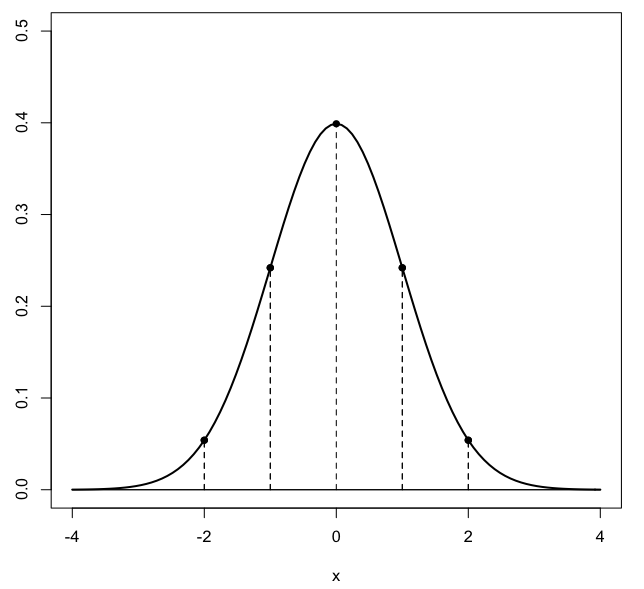
\includegraphics [scale=0.4] {gauss3.png} \end{center}

\begin{document}
\maketitle
\Large
\noindent
In the second volume of his \emph{Lectures on Physics}, Feynman has a great discussion of the principle he calls "least" or "stationary" action.  I want to follow his argument here. 

\begin{center} 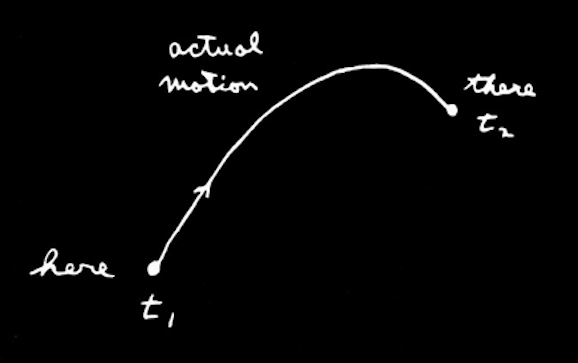
\includegraphics [scale=0.5] {feynman_action1.png} \end{center}
 
The basic principle is that the path followed by an object is such that it minimizes the difference between the kinetic and potential energy.  This turns out to be equivalent to Newton's Laws.

In mathematical language, the principle is that this integral

\[ \text{Action} = S = \int_{t_1}^{t_2} \ [ \ \frac{1}{2} m (\frac{dx}{dt})^2 - mgx \ ] \ dt \]

well, he says it's not a "minimum" but it is a critical point, where the linear approximation of how it changes for a little change in the path is zero.  There are only second order terms in the correction if we shift the path a little bit.

This reminds us of an ordinary minimization problem, but it is much more complicated.  The area uses what is called the calculus of variations.  Another example of a problem in this area is to find which curve of a given length encloses the most area.  You know that the answer is a circle, but you will need the calculus of variations to prove it.

Here is what we are going to do.  We will label the path with the least action as $\underline{x}$.  We will make a small perturbation to $\underline{x}$ such that

\[ x(t) = \underline{x}(t) + \eta(t) \] 
\[ \frac{dx}{dt} = \frac{d\underline{x}}{dt} + \frac{d\eta}{dt} \]

\begin{center} 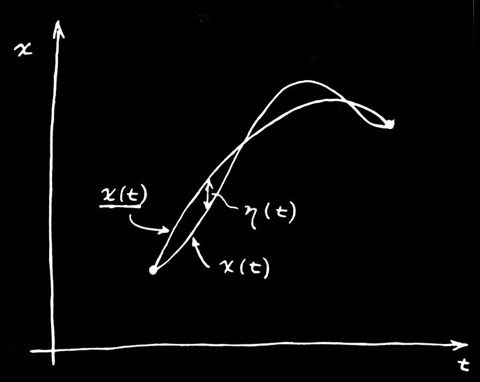
\includegraphics [scale=0.75] {feynman_action2.png} \end{center}

We write

\[ S = \int_{t_1}^{t_2} \ [ \ \frac{m}{2} (\frac{d\underline{x}}{dt} + \frac{d\eta}{dt})^2 - V(\underline{x} + \eta) \ ] \ dt \]
\[ (\frac{d\underline{x}}{dt} + \frac{d\eta}{dt})^2 = (\frac{d\underline{x}}{dt})^2 + 2 \frac{d\underline{x}}{dt}  \frac{d\eta}{dt} + ( \frac{d\eta}{dt})^2  \]

We will put any term involving $\eta^2$ into "a little box called 'second and higher order'" and not worry about it.

So the kinetic energy is

\[ \frac{m}{2} (\frac{d\underline{x}}{dt})^2 + m \frac{d\underline{x}}{dt}  \frac{d\eta}{dt} \]

We also have the potential energy

\[ V(\underline{x} + \eta) \]

We write a standard Taylor Series expansion ($\eta$ is small)

\[ V(\underline{x} + \eta) = V(x) + \eta V'(\underline{x}) + \frac{\eta^2}{2} V''(\underline{x}) + \dots \]

again neglecting second-order terms we have then

\[ V(\underline{x} + \eta) = V(x) + \eta V'(\underline{x}) \]

so

\[ S =  \int_{t_1}^{t_2} \ [ \  \frac{m}{2} (\frac{d\underline{x}}{dt})^2 + m \frac{d\underline{x}}{dt}  \frac{d\eta}{dt} - V(x) + \eta V'(\underline{x})  \ ] \ dt \]

We want to concentrate on the difference between this $S$ and $\underline{S}$, the path of least action.  Let's call that difference $\delta S$

\[ \delta S =  \int_{t_1}^{t_2} \ [ \  m \frac{d\underline{x}}{dt}  \frac{d\eta}{dt} -  \eta V'(\underline{x})  \ ] \ dt \]

Now, we are going to use integration by parts to make the derivative of $\eta$ disappear.

\[ \frac{d}{dt} (\eta f) = \eta \frac{df}{dt} + f \frac{d\eta}{dt} \]
\[  f \frac{d\eta}{dt} =  \frac{d}{dt} (\eta f) - \eta \frac{df}{dt} \]
\[  \int f \frac{d\eta}{dt} =  \int \frac{d}{dt} (\eta f) - \int \eta \frac{df}{dt} \]
\[  \int f \frac{d\eta}{dt} =  \eta f - \int \eta \frac{df}{dt} \]
\[  \int f \frac{d\eta}{dt} \ dt =  \eta f - \int \eta \frac{df}{dt} \ dt \]

In our problem

\[ f = m \frac{d \underline{x}}{dt} \]

We had 
\[ \delta S =  \int_{t_1}^{t_2} \ [ \  m \frac{d\underline{x}}{dt}  \frac{d\eta}{dt} -  \eta V'(\underline{x})  \ ] \ dt \]

and now we have
\[ \delta S =  m \frac{d \underline{x}}{dt} \eta(t) \bigg |_{t_1}^{t_2} - \int_{t_1}^{t_2}  \frac{d}{dt} (\  m \frac{d\underline{x}}{dt}) \ \eta(t) \ dt  -  \int_{t_1}^{t_2}  V'(\underline{x})   \eta(t) \ dt \]

Feynman says:  "Now comes something which always happens�the integrated part disappears."  The reason is that we must start and finish all the paths at the same place.  This means that $\eta$ is zero at both $t_1$ and $t_2$, and so the first term goes away.  We factor out the $\eta(t)$ in the rest of it to obtain

\[ \delta S =   \int_{t_1}^{t_2} \ [ \ -\frac{d}{dt} (\  m \frac{d\underline{x}}{dt}) - V'(\underline{x}) \ ] \  \eta(t) \ dt \]
\[ \delta S =   \int_{t_1}^{t_2} \ [ \ - m \frac{d^2\underline{x}}{dt^2} - V'(\underline{x}) \ ] \  \eta(t) \ dt \]

Our principle of least action says that $\delta S = 0$ for \emph{any} $\eta$.  So that means that what multiplies $\eta$ must be equal to zero.

\[ - m \frac{d^2\underline{x}}{dt^2} - V'(\underline{x})  \]
\[ - V'(\underline{x})  = m \frac{d^2\underline{x}}{dt^2}  \]
\[ - V'(\underline{x})  = m a  \]

and the force is the derivative of the potential with respect to position (with a minus sign), thus

\[ F  = m a  \]

There is a lot more in the lecture, but I will leave it at this.  Feynman closes this section by saying 

\quote{�One remark: I did not prove it was a minimum - maybe it's a maximum. In fact, it doesn't really have to be a minimum. It is quite analogous to what we found for the �principle of least time� which we discussed in optics. There also, we said at first it was �least� time. It turned out, however, that there were situations in which it wasn't the least time. The fundamental principle was that for any first-order variation away from the optical path, the change in time was zero; it is the same story. What we really mean by �least� is that the first-order change in the value of S, when you change the path, is zero. It is not necessarily a �minimum.�}



\end{document}  